\subsection{}

How much does the price and quantity of a product go up or down?
\begin{definition}
    \emph{Elasticity of Demand} is the measure of how much the quantity demanded changes when the price changes.
\end{definition}
Q: If price changes by 1\%, by how much does quantity demanded change (in \%)?\\
A: Price Elasticity of Demand($\eta$).\\
\begin{equation}
    \eta = \frac{\%\Delta Q}{\%\Delta P}=
    \frac{(Q_1 - Q_0)/Q_0}{(P_1 - P_0)/P_0}
    =\frac{Q_1 - Q_0}{P_1 - P_0} \cdot \frac{P_0}{Q_0}=\frac{1}{\text{Slope}}\cdot \frac{P_0}{Q_0}
\end{equation}
When working on price elasticity for demand, the answer is always negative.\\
\[
\eta = 
    \begin{cases}
        \eta = 0\; \text{Perfectly Inelastic}\; \text{e.g. Insulin}\\
        0 < \eta < 1\; \text{Inelastic}\; \text{e.g. Gasoline}\\
        \eta = 1\; \text{Unit Elastic}\; \text{e.g. Lander's mother buying lottery tickets}\\
        1 < \eta < \infty\; \text{Elastic}\; \text{e.g. Non-essential goods}\\
        \eta = \infty\; \text{Perfectly Elastic}\; \text{e.g. PC Cola}
    \end{cases}
\]
Elasticity changes as you move along a given demand curve.\\
There are three basic determinants of elasticity:
\begin{enumerate}
    \item Ceteris Paribus, The more substitutes the product has, the more elastic its demand is.
    \item Ceteris Paribus, the more of your budget this good takes up, the more elastic demand for it is.
    \item Ceteris Paribus, the more time you have to adjust, the more elastic your demand for the product will be.
\end{enumerate}
Elasticity is connected to how much a consumer spends on a product and much revenue a producer makes.
\begin{example}
    If price goes up, then total revenue\dots
    \begin{figure}[H]
        \centering
        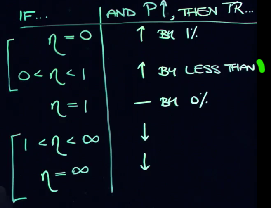
\includegraphics[]{Chapter4/PriceElasticityExamples.png}
        \caption{Price Elasticity Effects on Total Revenue}
    \end{figure}
\end{example}